\section{Pruebas del Sistema}

Este capítulo documenta la estrategia de pruebas aplicada al ecosistema Paralegales y la evidencia que la respalda. A diferencia del capítulo de desarrollo, que describe los componentes construidos, y del de resultados, que confronta los objetivos con la evidencia demostrativa obtenida, aquí el propósito es detallar cómo se verifica de forma sistemática que el sistema se comporta conforme a lo esperado, en particular allí donde un fallo silencioso tendría mayor impacto. La estrategia no persigue experimentación controlada, sino el aseguramiento de la confiabilidad de una plataforma en producción con base de usuarios activa, y combina una capa de pruebas automatizadas —centrada en el blindaje de los datos mediante las reglas de seguridad de Firestore— con una capa de validación manual sistemática sobre el entorno de \textit{staging}; se documentan además la evaluación exploratoria de pruebas \textit{end-to-end} y su integración en el \textit{pipeline} de integración continua.

\subsection{Enfoque y Estrategia de Pruebas}\label{subsec:enfoque-pruebas}

El alcance de las pruebas está determinado por dos restricciones del contexto: se interviene una plataforma en producción cuya estabilidad no puede comprometerse y el equipo de desarrollo es reducido. Por ello la estrategia no busca una cobertura uniforme de todo el sistema, sino una asignación del esfuerzo de verificación guiada por el riesgo, organizada en capas complementarias a modo de adaptación pragmática de la pirámide de pruebas:

\begin{itemize}
  \item \textbf{Pruebas unitarias automatizadas:} concentradas en las Reglas de Seguridad de Firestore —el mecanismo de control de acceso a los datos y, por tanto, el punto donde un error tendría consecuencias directas sobre la confidencialidad de la información—, ejecutadas de forma automática y repetible sobre un entorno emulado.

  \item \textbf{Validación manual sistemática:} ejercida sobre el entorno de \textit{staging}, donde se verifican de extremo a extremo los flujos funcionales críticos —incluida la interacción entre \textit{frontend}, servicios del lado del servidor e integraciones externas— antes de promover los cambios a producción.

  \item \textbf{Evaluación exploratoria de pruebas \textit{end-to-end}:} una iniciativa que valoró automatizar los flujos de interfaz pero que, por razones de costo-beneficio, no se consolidó.
\end{itemize}

En consonancia con el enfoque de evaluación de resultados (\autoref{subsec:enfoque-resultados}), la evidencia de este capítulo es demostrativa y artefactual —ejecuciones de la \textit{suite}, casos documentados y capturas del comportamiento observado—, no de carácter experimental.

\subsection{Pruebas Unitarias de las Reglas de Seguridad de Firestore}\label{subsec:pruebas-reglas-firestore}

El control de acceso a los datos en Paralegales se delega en las Reglas de Seguridad de Firestore, una capa declarativa que decide, para cada operación de lectura, escritura o eliminación, si la solicitud está autorizada en función de la identidad del usuario y del estado de los datos. Por ser la última línea de defensa frente a accesos indebidos, su corrección se valida mediante una \textit{suite} de pruebas unitarias automatizada y repetible.

\subsubsection{Entorno de ejecución y herramientas}

La \textit{suite} se construye con Vitest y la librería oficial \texttt{@firebase/rules-unit-testing}, y se ejecuta contra la \textit{Firebase Emulator Suite}, que despliega de forma local y efímera una instancia de Firestore sin incurrir en costos ni afectar entornos reales. La gestión del entorno se centraliza en dos utilidades: una de inicialización, que carga las reglas reales del archivo \texttt{firestore.rules} —de modo que se verifica exactamente el artefacto que se despliega—, siembra opcionalmente datos de partida con las reglas deshabilitadas y expone un contexto de ejecución \textbf{autenticado} o \textbf{no autenticado}; y otra que limpia los datos y libera el entorno tras cada caso, garantizando el aislamiento. Sobre Vitest se definieron además dos \textit{matchers} personalizados, \texttt{toAllow} y \texttt{toDeny} —apoyados en \texttt{assertSucceeds} y \texttt{assertFails}—, que permiten redactar aserciones legibles del tipo \textit{``el propietario puede leer su documento''} o \textit{``un usuario no puede leer el de otro''}.

\subsubsection{Diseño de casos: pruebas positivas y negativas}

La \textit{suite} se organiza por colección y, dentro de cada una, por tipo de operación, combinando casos positivos y negativos para certificar tanto que el acceso legítimo funciona como que el indebido se bloquea. Las baterías cubren las colecciones críticas del dominio: las \textbf{reglas básicas} (rechazo de lecturas sobre colecciones no autorizadas o de eliminaciones no contempladas), la colección \texttt{users} (aislamiento entre usuarios: cada uno solo lee y crea su propio documento), la colección \texttt{payments} (solo el propietario accede a sus pagos, y las actualizaciones de los flujos de proceso se rechazan ante un solicitante no propietario o datos inválidos) y la colección \texttt{associations} (reglas de listado según el estado de autenticación). La predominancia de casos negativos —solicitudes que \textit{deben} fallar— es deliberada: confirmar que el acceso indebido se bloquea es justo el tipo de regresión que una validación manual pasa por alto.

\subsubsection{Ejecución}

La \textit{suite} se ejecuta mediante el \textit{script} \texttt{test:rules}, que levanta el emulador de Firestore y corre las pruebas en su contexto con \texttt{firebase emulators:exec}. De este modo, cada ejecución parte de un entorno limpio y aislado, con resultados deterministas y reproducibles. La \autoref{fig:pruebas-rules-run} muestra una corrida de la \textit{suite}.

\newcommand\pruebasRulesRunCaption{Ejecución de la \textit{suite} de pruebas unitarias de las reglas de seguridad de Firestore sobre la \textit{Firebase Emulator Suite}. \hspace{1em}}
\begin{figure}[H]
  \centering
  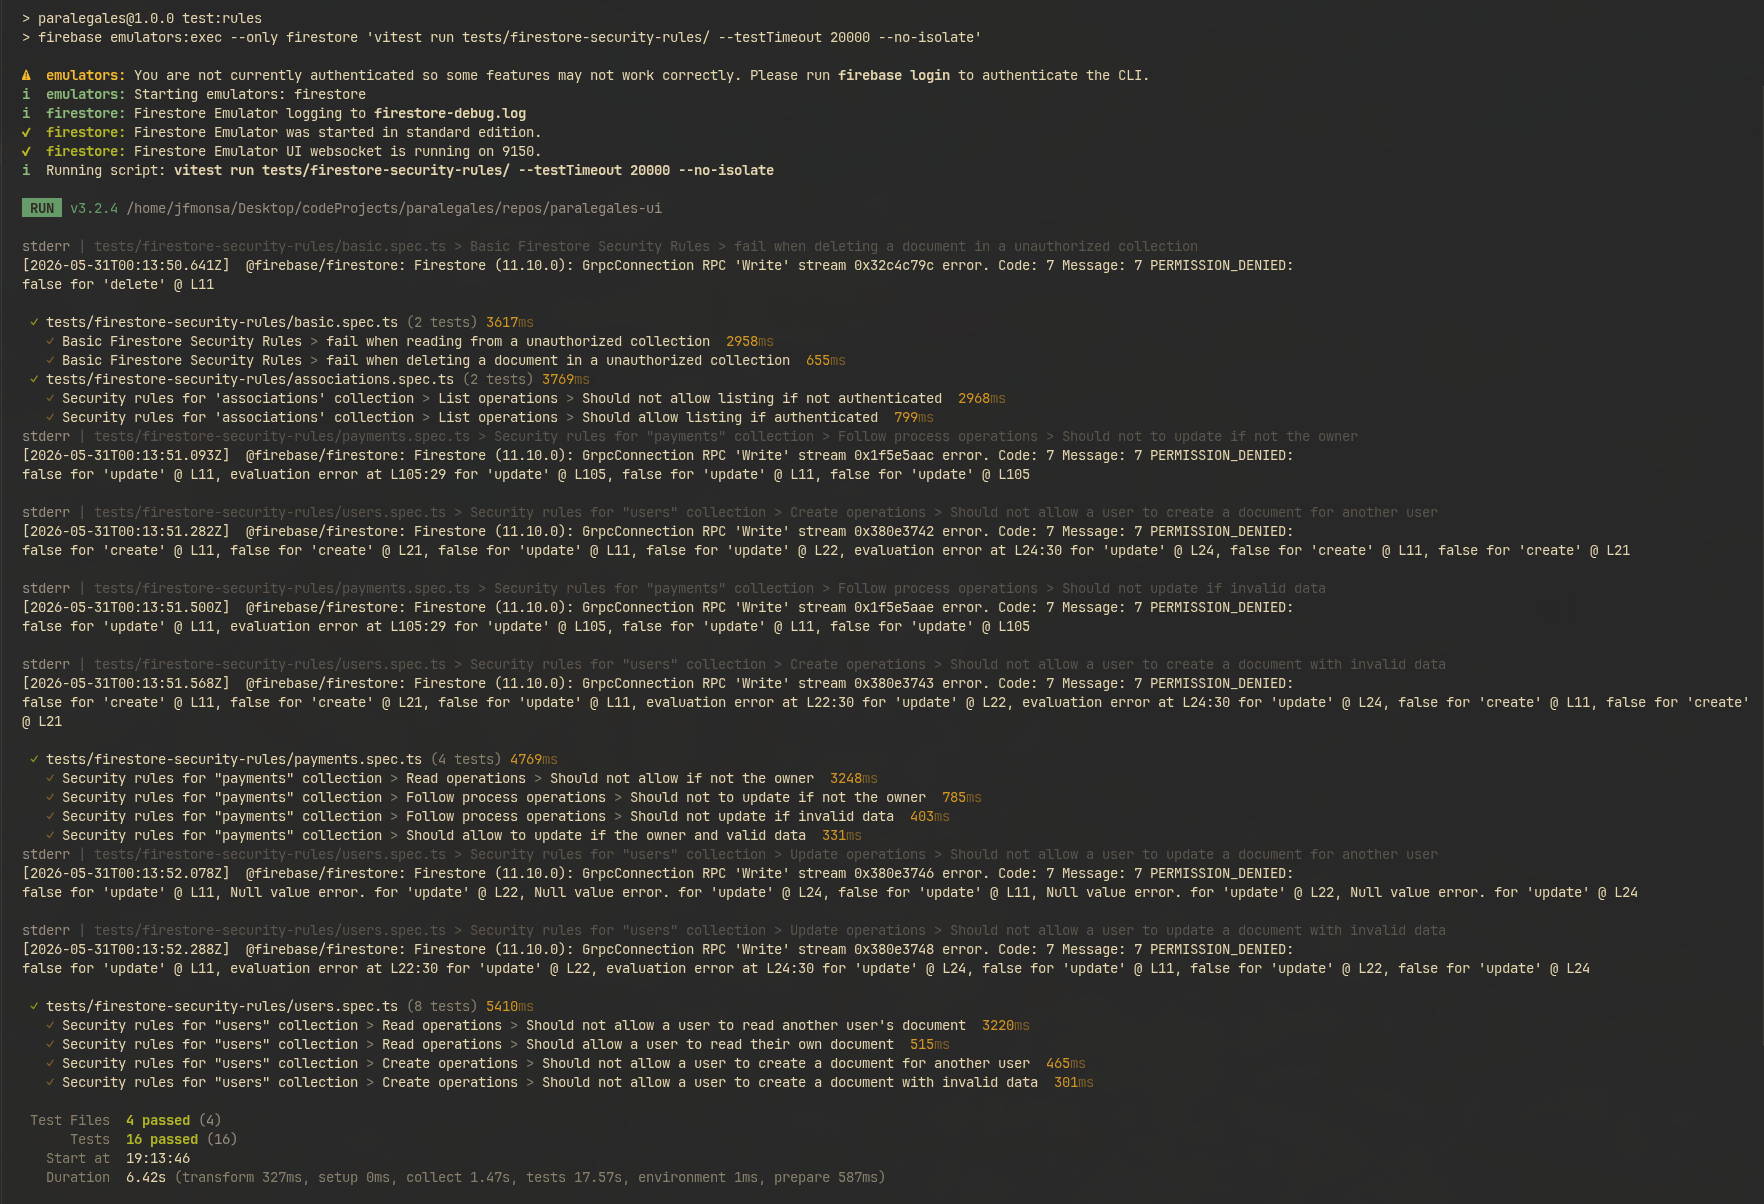
\includegraphics[width=1\textwidth]{img/figures/fig40-pruebas-rules-run.png}
  \caption[\pruebasRulesRunCaption]{\pruebasRulesRunCaption Fuente: Elaboración propia.}
  \label{fig:pruebas-rules-run}
\end{figure}

\subsection{Validación Manual Sistemática en el Entorno de \textit{Staging}}\label{subsec:validacion-manual}

Las pruebas de reglas aseguran un aspecto crítico pero acotado. La verificación de que los flujos funcionales operan correctamente de extremo a extremo —integrando el \textit{frontend}, los servicios del lado del servidor y las integraciones con terceros, como la API de la Rama Judicial— se realizó mediante validación manual sistemática sobre el entorno de \textit{staging} (\texttt{stage.paralegales.co}). Este entorno funciona como réplica de producción y compuerta de validación previa al despliegue: cada conjunto de cambios se despliega primero allí, sobre datos y condiciones representativos, lo que permite observar el comportamiento real del sistema —incluida la interacción con servicios externos y la experiencia de usuario— sin riesgo para los usuarios finales.

La validación combinó \textbf{pruebas de aceptación} de los flujos críticos de mayor valor de negocio —autenticación y registro, gestión de procesos y operación de campañas— siguiendo escenarios predefinidos con resultado esperado explícito, y \textbf{pruebas exploratorias} orientadas a descubrir comportamientos inesperados en los bordes de cada flujo. Para sistematizar la primera modalidad, los flujos se documentaron como casos de prueba con identificador, pasos y resultado esperado, ejecutables de forma consistente ante cada cambio relevante; la \autoref{tab:casos-manuales} recoge un conjunto representativo.

\newcommand\casosManualesCaption{Casos representativos de la validación manual sistemática ejecutada en \textit{staging}. \hspace{1em}}

\begingroup
\renewcommand{\arraystretch}{1.3}
\begin{longtable}{|p{1.6cm}|p{4.4cm}|p{5cm}|p{3.6cm}|}
  \hline
  \grayTableHeaderCell{1.6cm}{ID} &
  \grayTableHeaderCell{4.4cm}{Flujo} &
  \grayTableHeaderCell{5cm}{Escenario / pasos} &
  \grayTableHeaderCell{3.6cm}{Resultado esperado} \\
  \hline
  \endfirsthead

  \hline
  \grayTableHeaderCell{1.6cm}{ID} &
  \grayTableHeaderCell{4.4cm}{Flujo} &
  \grayTableHeaderCell{5cm}{Escenario / pasos} &
  \grayTableHeaderCell{3.6cm}{Resultado esperado} \\
  \hline
  \endhead

  \continuacionTablaFooter{4}
  \endfoot
  \endlastfoot

  \tableCell{CP-01} &
  \tableCell{Registro de usuario} &
  \tableCell{Registrar un usuario nuevo con datos válidos y verificación de teléfono.} &
  \tableCell{Cuenta creada y sesión iniciada; documento de usuario asociado al \texttt{uid}.} \\
  \hline

  \tableCell{CP-02} &
  \tableCell{Autenticación} &
  \tableCell{Iniciar sesión con credenciales válidas e inválidas.} &
  \tableCell{Acceso concedido con credenciales válidas; mensaje de error controlado en caso contrario.} \\
  \hline

  \tableCell{CP-03} &
  \tableCell{Consulta de procesos (Rama Judicial)} &
  \tableCell{Consultar un proceso a través del BFF que integra la API de la Rama Judicial.} &
  \tableCell{Datos del proceso recuperados y normalizados; errores de la fuente externa manejados sin exponer detalles internos.} \\
  \hline

  \tableCell{CP-04} &
  \tableCell{Seguimiento de proceso} &
  \tableCell{Activar el seguimiento de un proceso por parte del usuario propietario.} &
  \tableCell{Seguimiento registrado únicamente para el propietario; acceso ajeno bloqueado.} \\
  \hline

  \tableCell{CP-05} &
  \tableCell{Operación de campañas} &
  \tableCell{Crear y ejecutar una campaña sobre el módulo correspondiente.} &
  \tableCell{Campaña creada y procesada conforme a la lógica del lado del servidor.} \\
  \hline

  \tableCell{CP-06} &
  \tableCell{Aislamiento de datos} &
  \tableCell{Intentar acceder a información de otro usuario desde una sesión distinta.} &
  \tableCell{Acceso denegado, en consistencia con las reglas de seguridad de Firestore.} \\
  \hline

  \caption[\casosManualesCaption]{\casosManualesCaption Fuente: Elaboración propia.}
  \label{tab:casos-manuales}
\end{longtable}
\endgroup

Este proceso, aunque manual, fue sistemático y repetible, y constituyó el principal mecanismo de aseguramiento funcional de extremo a extremo del proyecto; sus limitaciones se analizan en la síntesis del capítulo (\autoref{subsec:sintesis-pruebas}).

\subsection{Evaluación Exploratoria de Pruebas \textit{End-to-End}}\label{subsec:evaluacion-e2e}

Durante una fase exploratoria se evaluó incorporar pruebas \textit{end-to-end} (E2E) con Playwright sobre los emuladores locales de Firestore y Authentication, para valorar la viabilidad de automatizar los recorridos de interfaz verificados hasta entonces de forma manual. La exploración estructuró los cimientos de una \textit{suite} —configuración contra los emuladores, patrón \textit{Page Object Model}, \textit{fixtures} para preparar el estado de Firebase y casos iniciales de inicio de sesión y registro—, pero su adopción se mantuvo a un nivel mínimo y no se consolidó como parte de la \textit{suite} oficial del proyecto.

La decisión respondió a un criterio de costo-beneficio: las pruebas E2E de interfaz son las más costosas de mantener de la pirámide —sensibles a cambios de interfaz, propensas a fallos intermitentes y de mantenimiento sostenido—, difíciles de absorber por un equipo reducido sin desplazar esfuerzo de las funcionalidades prioritarias. Por ello se concentró la automatización en la capa de mayor riesgo y menor volatilidad —las reglas de seguridad— y se sostuvo la validación de extremo a extremo con el proceso manual descrito. Documentar esta evaluación responde a un criterio de transparencia: dejó una base reutilizable para una futura consolidación de la \textit{suite} E2E, posibilidad que se retoma en el trabajo futuro.

\subsection{Integración de las Pruebas en el \textit{Pipeline} de Integración Continua}\label{subsec:pruebas-ci}

El valor de una \textit{suite} de pruebas se maximiza cuando su ejecución es automática y obligatoria, de modo que ninguna integración degrade las garantías ya verificadas. El \textit{pipeline} de integración continua en GitHub Actions —descrito en el capítulo de desarrollo (\autoref{subsec:sdlc}) y evidenciado en el de resultados (\autoref{subsec:resultado-d})— se ejecuta de forma obligatoria frente a cada \textit{pull request} dirigida a las ramas protegidas, aplicando dos compuertas de calidad: la validación estática diferencial (\textit{linting} y formato sobre los archivos modificados) y la ejecución automática de la \textit{suite} de reglas de seguridad, para la cual aprovisiona la \textit{Firebase Emulator Suite} y corre el \textit{script} \texttt{test:rules} contra el emulador de Firestore.

Así, la garantía de seguridad deja de depender de una acción manual y se convierte en una compuerta automática del proceso de integración: una \textit{pull request} cuyas modificaciones rompan una regla de seguridad es bloqueada antes de promoverse, evitando que una regresión en el blindaje de los datos alcance \textit{staging} o producción. Mejoras incrementales como el cacheo del emulador y la publicación de artefactos de cobertura se retoman en el apartado de trabajo futuro.

\subsection{Síntesis y Limitaciones}\label{subsec:sintesis-pruebas}

La estrategia de pruebas del proyecto se asienta en una asignación del esfuerzo guiada por el riesgo, antes que en una cobertura uniforme. La \autoref{tab:sintesis-pruebas} resume las capas de validación, su grado de automatización y la evidencia que las respalda.

\newcommand\sintesisPruebasCaption{Síntesis de las capas de la estrategia de pruebas. \hspace{1em}}

\begingroup
\renewcommand{\arraystretch}{1.3}
\begin{longtable}{|p{4.5cm}|p{3cm}|p{6.5cm}|}
  \hline
  \grayTableHeaderCell{4.5cm}{Capa de validación} &
  \grayTableHeaderCell{3cm}{Automatización} &
  \grayTableHeaderCell{6.5cm}{Evidencia / estado} \\
  \hline
  \endfirsthead

  \hline
  \grayTableHeaderCell{4.5cm}{Capa de validación} &
  \grayTableHeaderCell{3cm}{Automatización} &
  \grayTableHeaderCell{6.5cm}{Evidencia / estado} \\
  \hline
  \endhead

  \continuacionTablaFooter{3}
  \endfoot
  \endlastfoot

  \tableCell{Reglas de seguridad de Firestore} &
  \tableCell{Automatizada} &
  \tableCell{\textit{Suite} con Vitest sobre la \textit{Firebase Emulator Suite}; casos positivos y negativos por colección; ejecutada como compuerta obligatoria en el \textit{pipeline} de CI (\autoref{subsec:pruebas-ci}).} \\
  \hline

  \tableCell{Flujos funcionales de extremo a extremo} &
  \tableCell{Manual} &
  \tableCell{Validación sistemática y exploratoria en \textit{staging}; casos documentados (\autoref{tab:casos-manuales}).} \\
  \hline

  \tableCell{Pruebas \textit{end-to-end} de interfaz} &
  \tableCell{Exploratoria, no consolidada} &
  \tableCell{Base montada con Playwright (POM y \textit{fixtures}); no adoptada por costo-beneficio.} \\
  \hline

  \tableCell{Validación estática (\textit{lint} / formato)} &
  \tableCell{Automatizada} &
  \tableCell{Compuerta obligatoria en el \textit{pipeline} de CI sobre archivos modificados (\autoref{subsec:sdlc}).} \\
  \hline

  \caption[\sintesisPruebasCaption]{\sintesisPruebasCaption Fuente: Elaboración propia.}
  \label{tab:sintesis-pruebas}
\end{longtable}
\endgroup

\subsubsection{Limitaciones}

El reconocimiento explícito de las limitaciones es parte del rigor con que se presenta la estrategia: la automatización se concentra en las reglas de seguridad, mientras que la lógica de negocio del lado del servidor y los flujos de interfaz carecen de una \textit{suite} automatizada equivalente y dependen de la validación manual; esta, a su vez, recae en el esfuerzo humano, lo que la hace sensible a la disponibilidad del equipo y menos exhaustiva ante regresiones sutiles. Por su parte, la automatización de los flujos \textit{end-to-end} quedó en estado exploratorio.

\subsubsection{Trabajo futuro}

De estas limitaciones se derivan líneas de mejora directas: (i) optimizar la ejecución de la \textit{suite} de reglas en CI mediante el cacheo del emulador y la publicación de artefactos de cobertura; (ii) consolidar la \textit{suite} \textit{end-to-end} con Playwright sobre la base ya construida, priorizando los flujos críticos de mayor estabilidad; y (iii) extender la automatización hacia la lógica de negocio del lado del servidor. Estas mejoras trasladarían parte de la carga de validación manual hacia mecanismos automáticos y continuos, fortaleciendo el aseguramiento de calidad a medida que el sistema crece.

